
%\chapter{Appendix}

\chapter{Additional remarks on elasticity theory and FE methods} 

\section{Basics of vector analysis} 

\subsection{Divergence theorem}
\label{ADivergenceTheorem}
For any smooth vector field $\mv(\mbx)$ and any smooth tensor field $\mathbf{A}(\mbx)$ that are defined on a compact region $\Omega$ which is enclosed by the smooth, closed surface $\partial \Omega$ we have
\begin{eqnarray}
\int _{\partial \Omega} \mv \cdot \mn \mdA = \int _{\Omega} \mdiv \mv \mdV \qquad \textnormal{or} \qquad \int _{\partial \Omega} v_i n_i \mdA = \int _{\Omega} \frac{\partial v_i}{\partial x_i} \mdV
\end{eqnarray}

\begin{eqnarray}
\int _{\partial \Omega} \mathbf{A}  \mn \mdA = \int _{\Omega} \mdiv \mathbf{A} \mdV \qquad \textnormal{or} \qquad \int _{\partial \Omega} A_{ij} n_j \mdA = \int _{\Omega} \frac{\partial A_{ij}}{\partial x_j} \mdV
\end{eqnarray}

\subsection{Product differentiation rules for tensors}
\label{AProductRule}
For any smooth vector field $\mv(\mbx)$ and any smooth tensor field $\mathbf{A}(\mbx)$ we have

\begin{eqnarray}
\mdiv(\mathbf{A}^T \mv) = \mdiv(\mathbf{A}) \cdot \mv + \mdiv(\mathbf{A}) : \mgrad( \mv)
\end{eqnarray}

\section{Work conjugancy of $\mbS$ and $\dot{\mbE}$} 
\label{WorkConjugancySE}

It has already been shown in section (\ref{SectionMechanicalEnergyInElasticBodies}) that the first Piola-Kirchhoff stress tensor $\mbP$ is work conjugated to the material time derivative of the deformation gradient $\mbF$. It is quickly shown that the material time derivative of the Cauchy-Green strain tensor $\mbC$
\begin{alignat}{1}
\dot \mbC = \mddt \left( \mbF ^T \mbF \right) = \mbdotF ^T \mbF + \mbF ^T \mbdotF
\end{alignat}
related to the material time derivative of the Green-Lagrange strain tensor by
\begin{alignat}{1}
\dot \mbE = \mddt \frac{1}{2} \left( \mbF ^T \mbF  - \mbI\right) = \frac{1}{2} \left( \mbdotF ^T \mbF + \mbF ^T \mbdotF \right) = \frac{1}{2} \dot \mbC.
\end{alignat}

Based on the results of section \ref{SectionMechanicalEnergyInElasticBodies} (work conjugancy of $\mbP$ and $\mbdotF$), we can thus derive 
\begin{alignat}{1}
\mbP : \mbdotF  &= \mtr(\mbP ^T \mbdotF) = \mtr(\mbdotF ^T \mbP) = \mtr(\mbdotF ^T \mbF \underbrace{ \mbF ^{-1} \mbP}_{\mbS}) \\
&= \mtr(\mbS \mbdotF^T \mbF) =  \mtr(\mbS \mbF \mbdotF^T ) = \mtr(\mbS \frac{1}{2}(\mbdotF^T \mbF +  \mbF \mbdotF^T )) \\
&= \frac{1}{2} \mbS: \dot{\mbC} = \mbS: \dot{\mbE}
\end{alignat}

\section{The Saint Venant-Kirchhoff model} 
\label{ASVKModel}

The elastic energy functional for Saint-Venant Kirchhoff model is defined by
 \begin{equation}
 \mPsi  (\mbE )  = \frac{\lambda}{2} (\mtr \mbE)^2 + \mu \mtr (\mbE^2).
\end{equation}

In order to express the relation 
 \begin{equation}
 \mbS (\mbE) = \frac{ \partial \mPsi  (\mbE )}{\partial \mbE},
\end{equation}

we note the partial derivatives 

 \begin{equation}
\frac{\partial \mtr (\mbE)}{\partial \mbE} = \frac{1}{\partial E_{ij}} \sum_{k=1} ^3 E_{kk} = \delta_{ij} = \mbI
\end{equation}

and

 \begin{equation}
 \mbS (\partial \mbE) = \frac{\partial \mtr (\mbE^2)}{\partial \mbE} = \frac{1}{\partial E_{ij}} \sum_{k,l=1} ^3 E_{kl} E_{kl} = 2 E_{ij} = 2 \mbE.
\end{equation}

Thus, we obtain

 \begin{equation}
\frac{ \partial \mPsi  (\mbE )}{\partial \mbE} = \frac{\lambda}{2} \frac{ \partial \left( (\mtr \mbE)^2 \right)}{\partial \mbE } + \mu \frac{ \partial \left( \mtr (\mbE^2) \right) }{\partial \mbE} = \lambda \mtr{\mbE} \mbI + 2 \mu \mbE.
\end{equation}

\section{Polynomial shape functions for selected elements} 
\label{AShapeFunctions}

\begin{figure}
   \centering   
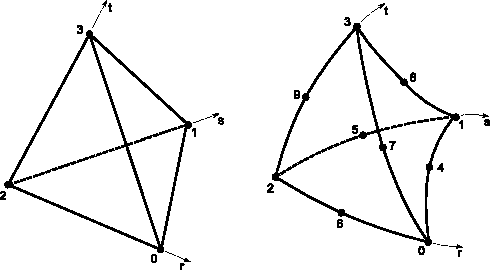
\includegraphics[width=8.5cm]{Figures/Tet4and10.pdf}
\caption{Linear tetrahedron with 4 nodes (tet4) and quadratic tetrahedron with 10 nodes (tet10)}
\label{TetraAppendix}
\end{figure}

\subsection{Nodal shape functions in local (curvilinear) coordinates}
Linear 4-node tetrahedron (node numbering as shown in Fig. \ref{TetraAppendix}):
\begin{alignat}{1}
N_0(r,s,t) &= r\\ 
N_2(r,s,t) &= s\\
N_3(r,s,t) &= 1-r-s-t\\
N_4(r,s,t) &= t\\
\end{alignat}

Quadratic 10-node tetrahedron (node numbering as shown in Fig. \ref{TetraAppendix}):
\begin{alignat}{1}
N_0(r,s,t) &= (2r-1)r\\ 
N_1(r,s,t) &= (2s-1)s\\
N_2(r,s,t) &= (2 (1-r-s-t) -1)(1-r-s-t)\\
N_3(r,s,t) &= (2t-1)t\\
N_4(r,s,t) &= 4rs\\
N_5(r,s,t) &= 4(1-r-s-t)s\\
N_6(r,s,t) &= 4(1-r-s-t)r\\
N_7(r,s,t) &= 4st\\
N_8(r,s,t) &= 4rt\\
N_9(r,s,t) &= 4(1-r-s-t)t\\
\end{alignat}

\subsection{Nodal shape functions in global coordinates}

The standard triangle [(1,0,0) (0,1,0) (0,0,0) (0,0,1)] is mapped to the global coordinate system using the shape functions (isometric elements). If $\mathbf X_k$ denotes the initial position of the k-th node of the n-node tetrahedron, we define the function $\xi(\mathbf r)$ that maps the local coordinates $\mathbf r = (r,s,t)$ to the global coordinates $\mbX = (X_1, X_2,X_3)$:
\begin{equation}
\xi (\mathbf {r}) = \mbX (\mathbf{ r}) = \mbX (r,s,t) = \sum_{k=0} ^n \mbX _k N_k(r,s,t)
\end{equation}

The global derivatives of the shape functions are
\begin{equation}
\frac{\partial N_I(\mbx)}{\partial \mbX} = \mathbf J^{-1} \frac{\partial N_I(\mbx)}{\partial \mathbf r}
\end{equation}

where $\mathbf J$ is the jacobian
\begin{equation}
\mathbf J = \nabla \xi = \left(
\begin{array}{ccc}
\frac{\partial X_1}{\partial r} & \frac{\partial X_2}{\partial r} & \frac{\partial X_3}{\partial r}\\
\frac{\partial X_1}{\partial s} & \frac{\partial X_2}{\partial s} & \frac{\partial X_3}{\partial s}\\
\frac{\partial X_1}{\partial t} & \frac{\partial X_2}{\partial t} & \frac{\partial X_3}{\partial t}
\end{array}
\right)
\end{equation}




\section{Internal nodal forces and the stiffness matrix for linear elasticity} \label{ANodalForces}

As detailed in section \ref{SectionMatrixFormulation}, the internal nodal forces are given by

\begin{eqnarray}
\mfint = \mfintThree = \mIntRConf \mfintDens \mdVZero = \sum_{e} \mIntREl \mfintDens \mdVZero = \mIntRConf \msigma_{ik}  \left( \nabla \mtfTwo \right)_{kI} \mdVZero.
\end{eqnarray}

By noting that the gradient of the displacement vector reads
\begin{eqnarray}
\nabla \mbu = \nabla (\mcu _I \mtf ) =  \mcu _I \nabla \mtf = \mcu _{iI} \left( \nabla \mtfTwo \right)_{kI},
\end{eqnarray}

we can express its the derivative with respect to the nodal displacements through
\begin{eqnarray}
\frac{\partial}{\partial \mcu _{jJ}} \left( \nabla \mcu \right)_{ik}  = \frac{\partial}{\partial \mcu _{jJ}} \left( \mcu _{iI} \left( \nabla \mtfTwo \right)_{kI} \right) = \delta _{ij} (\nabla \mtfTwo_{kJ}).
\end{eqnarray}


The derivative of the Cauchy strain with respect to the nodal displacements can thus be derived as
\begin{eqnarray}
\frac{\partial \meps _{ik}}{\partial \mcu _{jJ}} &=& \frac{1}{2} \frac{\partial}{\partial \mcu _{jJ}} \left( \nabla \mbu + (\nabla \mbu )^T \right) \notag \\
&=& \frac{1}{2} \frac{\partial}{\partial \mcu _{jJ}} \left(  \mcu _{iI} \left( \nabla \mtfTwo \right)_{kI}  + \mcu _{kI} \left( \nabla \mtfTwo \right)_{iI} \right) \notag \\
&=& \frac{1}{2}  \left( \delta _{ij} (\nabla \mtfTwo)_{kJ} + \delta _{kj} (\nabla \mtfTwo)_{iJ} \right).
\end{eqnarray}

Consequently, the derivation of the Cauchy stress follows as
\begin{eqnarray}
\frac{\partial \msigma _{ik}}{\partial \mcu _{jJ}} &=& 2\mu \frac{\partial \meps_{ik}}{\partial \mcu _{jJ}} + \lambda \delta _{ik} \frac{\partial \meps_{ll}}{\partial \mcu _{jJ}} \notag \\
&=& \mu \left( \delta _{ij} (\nabla \mtfTwo)_{kJ} + \delta _{kj} (\nabla \mtfTwo)_{iJ} \right) + \frac{\lambda}{2}  \delta _{ik} \left( \delta _{lj} (\nabla \mtfTwo)_{lJ} + \delta _{lj} (\nabla \mtfTwo)_{lJ} \right) \notag \\
&=& \mu \left( \delta _{ij} (\nabla \mtfTwo)_{kJ} + \delta _{kj} (\nabla \mtfTwo)_{iJ} \right) + \frac{\lambda}{2} 2 \delta _{ik} (\nabla \mtfTwo)_{jJ} \notag \\
&=& \mu \delta _{ij} (\nabla \mtfTwo)_{kJ} + \mu \delta _{kj} (\nabla \mtfTwo)_{iJ}  + \lambda \delta _{ik} (\nabla \mtfTwo)_{jJ} 
\end{eqnarray}

and the derivative of the internal force density can be expressed as
\begin{eqnarray}
\frac{\partial \mfintDens}{\partial \mcu _{jJ}} &=& \frac{\partial}{\partial \mcu _{jJ}} \left( \msigma_{ik}  \left( \nabla \mtfTwo \right)_{kI} \right) \mdVZero \notag \\
&=&  \frac{\partial \msigma_{ik}}{\partial \mcu _{jJ}} \left( \nabla \mtfTwo \right)_{kI}  \notag \\
&=& \left( \mu \delta _{ij} (\nabla \mtfTwo)_{kJ} + \mu \delta _{kj} (\nabla \mtfTwo)_{iJ}  + \lambda \delta _{ik} (\nabla \mtfTwo)_{jJ} \right) \left( \nabla \mtf \right)_{kI}  \notag \\
&=& \left( \mu \delta _{ij} (\nabla \mtfTwo)_{kJ} + \mu \delta _{kj} (\nabla \mtfTwo)_{iJ}  + \lambda \delta _{ik} (\nabla \mtfTwo)_{jJ} \right) \left( \nabla \mtf \right)_{kI}  \notag \\
&=&   \mu \delta _{ij} (\nabla \mtfTwo)_{kJ} \left( \nabla \mtf \right)_{kI} + \mu (\nabla \mtfTwo)_{iJ} \left( \nabla \mtf \right)_{jI} \notag \\
& & + \lambda  (\nabla \mtfTwo)_{jJ} \left( \nabla \mtf \right)_{iI}.
\end{eqnarray}

This yields the stiffness matrix
\begin{eqnarray}
\frac{\partial \mfintThree}{\partial \mcu _{jJ}} = \mIntRConf \frac{\partial \mfintDens}{\partial \mcu _{jJ}} \mdVZero = \sum_{e} \mIntREl \frac{\partial \mfintDens}{\partial \mcu _{jJ}} \mdVZero = \sum_{e} \mathbf{K}^e =  \msmat.
\end{eqnarray}

\section{Internal nodal forces and the stiffness matrix for corotated elasticity} \label{ACorotNodalForces}

The polar decomposition of deformation gradient (see section \ref{SectionPolarDecomposition})

\begin{eqnarray}
\mathbf F = \mathbf R \mathbf U
\end{eqnarray}

is used to define the stretch measure
\begin{eqnarray}
\mathbf U = \mathbf {R} ^T \mathbf F.
\end{eqnarray}

We express the displacement gradient through the nodal positions 
\begin{eqnarray}
\nabla \mbu = \mbF - \mbI = \nabla ( \mcx_J  \mbf ) =  \mcx_J  \nabla  \mbf - \mbI
\end{eqnarray}

in order to relate the Cauchy strain to the nodal positions:
\begin{eqnarray}
\meps &=& \frac{1}{2} \left( (\mbF - \mbI ) + (\mbF - \mbI  )^T \right)  = \frac{1}{2} \left( (\mcx_J  \nabla  \mbf - \mbI)+ (\mcx_J  \nabla  \mbf - \mbI )^T \right)  \notag \\
&=& \frac{1}{2} \left( \mcx_{iJ} (\nabla \mtfn)_{jJ} +  \mcx_{jJ} (\nabla \mtfn)_{iJ} \right) - \mbI.
\end{eqnarray}

For corotated elasticity, the deformation gradient is replaced by the stretch measure
\begin{equation}
\mSt = \mrot^T \nabla \mbF = R_{ki} \mcx_{kJ}  (\nabla \mtfn)_{jJ}.
\end{equation}



Consequently, the corotated Cauchy strain reads
\begin{eqnarray}
\meps ^{CR} &=& \meps_{ij} ^{CR} = \frac{1}{2} \left( \mrot^T \mcx_J \nabla \mbf +  (\mrot^T \mcx_J \nabla \mbf)^T \right) - \mbI
\end{eqnarray}

and the corotated stress is derived to
\begin{eqnarray}
\msigma_{ij} ^{CR} &=& 2\mu \meps^{CR}_{ij} + \lambda \delta _{ij} \meps^{CR}_{ll} \notag.
\end{eqnarray}

We note that the internal nodal forces can be written in terms of the variation of nodal position 
\begin{eqnarray}
D_{\delta \mcu} \meFunc (\mbu _h) _{int} &=& \mIntRConf \msigma : \delta \meps  \mdVZero =  \mIntRConf \msigma : \frac{1}{2} \left( \delta \nabla \mbu + (\delta \nabla \mbu)^T \right)  \mdVZero \notag\\
&=&  \mIntRConf \msigma :  \delta \nabla \mbu  \mdVZero = \mIntRConf \msigma : \left( \delta \mcu_I \nabla \mtf \right) \mdVZero \notag\\
&=& \mIntRConf \msigma : \left( \delta \mcx_I \nabla \mtf \right) \mdVZero
\end{eqnarray}

in order to derive the corotated nodal forces
\begin{eqnarray}
D_{\delta \mcu} \meFunc (\mbu _h) _{int} &=& \mIntRConf \msigma : \left( \mrot^T \delta \mcx_I \nabla \mtf \right) \mdVZero = \mIntRConf (\mrot \msigma) : \left(  \delta \mcx_I \nabla \mtf \right) \mdVZero \notag \\
&=& \delta \mcx_{iI} \mIntRConf \mrot_{im} \msigma_{mk}  (\nabla \mtfTwo)_{kI} \mdVZero = \delta \mcx_{iI} \mIntRConf \mfintDensCR \mdVZero  \notag \\
&=& \delta \mcx_{iI} \mfintThreeCR= \delta \mcx_I \mfintTwoCR
\end{eqnarray}

with
\begin{eqnarray}
\mfintDensCR =   \mIntRConf \mrot_{im} \msigma^{CR}_{mk}  (\nabla \mtfTwo)_{kI} \mdVZero.
\end{eqnarray}

In order to formulate the corotated stiffness matrix, we first compute the derivate of the corotated Cauchy strain with respect to the nodal positions:
\begin{eqnarray}
\frac{\partial \meps _{mk}}{\partial \mcx _{jJ}} &=& \frac{1}{2} \frac{\partial}{\partial \mcx _{jJ}} \left(R_{nm} F_{nk} + F_{nm} R_{nk}  \right) - \mbI \notag \\
&=& \frac{1}{2} \frac{\partial}{\partial \mcx _{jJ}} \left(R_{nm} \mcx_{nI} \left( \nabla \mtfTwo \right)_{kI}  + \mcx_{nI} \left( \nabla \mtfTwo \right)_{mI} R_{nk}  \right) \notag \\
&=& \frac{1}{2}  \left( \delta_{nj} R_{nm}  \left( \nabla \mtfTwo \right)_{kJ}  + \delta_{nj}\left( \nabla \mtfTwo \right)_{mJ} R_{nk}  \right) 
\end{eqnarray}

In a similar fashion as in the linear elastic case we derive
\begin{alignat}{1}
& \frac{\partial \msigma^{CR} _{mk}}{\partial \mcx _{jJ}} = 2\mu \frac{\partial \meps^{CR}_{mk}}{\partial \mcx _{jJ}} + \lambda \delta _{mk} \frac{\partial \meps^{CR}_{ll}}{\partial \mcx _{jJ}} \notag \\
&= \mu \left(  \delta_{nj} R_{nm}  \left( \nabla \mtfTwo \right)_{kJ}  + \delta_{nj}\left( \nabla \mtfTwo \right)_{mJ} R_{nk}  \right) \notag \\
& + \frac{\lambda}{2}  \delta _{mk} \left( \delta_{nj} R_{nl}  \left( \nabla \mtfTwo \right)_{lJ}  + \delta_{nj}\left( \nabla \mtfTwo \right)_{lJ} R_{nl}  \right)  \notag \\
&= \mu \left(  \delta_{nj} R_{nm}  \left( \nabla \mtfTwo \right)_{kJ}  + \delta_{nj}\left( \nabla \mtfTwo \right)_{mJ} R_{nk}  \right) + \lambda  \delta _{mk}  \delta_{nj} R_{nl}  \left( \nabla \mtfTwo \right)_{lJ}
\end{alignat}

and express the corotated force density through
\begin{eqnarray}
& &\frac{\partial \mfintDens}{\partial \mcx _{jJ}} = \frac{\partial}{\partial \mcx _{jJ}}  \mrot_{im} \msigma^{CR}_{mk}   \left(  \nabla \mtfTwo \right)_{kI} = \mrot_{im} \frac{\partial \msigma^{CR}_{mk}}{\partial \mcx _{jJ}}    \left(  \nabla \mtfTwo \right)_{kI} \notag \\
&=&   \mrot_{im} \left( \mu \left(  \delta_{nj} R_{nm}  \left( \nabla \mtfTwo \right)_{kJ}  + \delta_{nj}\left( \nabla \mtfTwo \right)_{mJ} R_{nk}  \right) + \lambda  \delta _{mk}  \delta_{nj} R_{nl}  \left( \nabla \mtfTwo \right)_{lJ}  \right)   \left(  \nabla \mtfTwo \right)_{kI}  \notag \\
&=& \mrot_{im}   \mu \left(  \delta_{nm} R_{jn}  \left( \nabla \mtfTwo \right)_{kJ} \left(  \nabla \mtfTwo \right)_{kI} + \left( \nabla \mtfTwo \right)_{mJ} R_{jk} \left(  \nabla \mtfTwo \right)_{kI} \right) \notag \\
& &+ \lambda    R_{jl}  \left( \nabla \mtfTwo \right)_{lJ} \left(  \nabla \mtfTwo \right)_{mI}   \notag \\
&=& \mrot_{im}   \mu \left(  \delta_{nm}   \left( \nabla \mtfTwo \right)_{kJ} \left(  \nabla \mtfTwo \right)_{kI} R_{jn} + \left( \nabla \mtfTwo \right)_{mJ}  \left(  \nabla \mtfTwo \right)_{nI} \right) R_{jn} \notag \\
& &+ \lambda     \left( \nabla \mtfTwo \right)_{nJ} \left(  \nabla \mtfTwo \right)_{mI}  R_{jn}  \notag \\
&=& \mrot_{im}   \left( \mu \left(  \delta_{nm}   \left( \nabla \mtfTwo \right)_{kJ} \left(  \nabla \mtfTwo \right)_{kI}  + \left( \nabla \mtfTwo \right)_{mJ}  \left(  \nabla \mtfTwo \right)_{nI} \right) + \lambda     \left( \nabla \mtfTwo \right)_{nJ} \left(  \nabla \mtfTwo \right)_{mI} \right) R_{jn}  \notag \\
&=& \mrot_{im}  \frac{\partial \hat{f}  ^{int}_{mI} }{\partial \mcx _{nJ}}   R_{jn} = \mathbf{R}  \frac{\partial \mfintTwoCR }{\partial \mcx _{J}}   \mathbf{R}^T .
\end{eqnarray}

The global corotated stiffness matrix is then given by
\begin{eqnarray}
\msmat ^{CR} =  \sum_{e} \mIntREl \frac{\partial \mfintDens}{\partial \mcx _{jJ}} \mdVZero = \sum_{e} \mIntREl  \mathbf{R}  \frac{\partial \mfintDensTwo }{\partial \mcx _{J}}   \mathbf{R}^T \mdVZero. 
\end{eqnarray}

%Similarly, we can derive the tangent stiffness for $\mthZero \mcx$:
%\begin{eqnarray}
%\mthZero \msmat_{IJ}  = \mthZero \msmat_{iIjJ}  =  \sum_{e} \mIntREl \frac{\partial \mfintDens}{\partial \mthZero \mcx  _{jJ}} \mdVZero  &=&  \sum_{e} \mIntREl  \mrot_{im}  \frac{\partial \hat{f}  ^{int}_{mI} }{\partial \mthZero \mcx  _{nJ}}  \mdVZero = \sum_{e} \mIntREl  \mathbf{R}  \frac{\partial \mfintDensTwo }{\partial \mthZero \mcx   _{J}}  \mdVZero  
%\end{eqnarray}
%
%Consequently the internal forces can be described as:
%\begin{eqnarray}
%\mfint_{I} = \msmat_{IJ}^{CR} \mcx  _{J} - \mthZero \msmat_{IJ}^{CR} \mthZero \mcx  _{J}
%\end{eqnarray}




